\documentclass[11pt,a4paper]{article}
\usepackage[margin=2.2cm]{geometry}
\usepackage[T1]{fontenc}
\usepackage{lmodern}
\usepackage{tikz}
\usetikzlibrary{arrows.meta,positioning,calc}
\usepackage{booktabs}
\usepackage{longtable}
\usepackage{array}
\usepackage{xcolor}
\usepackage{enumitem}
\usepackage{url}
\usepackage{hyperref}
\hypersetup{colorlinks=true,linkcolor=black,urlcolor=blue!50!black}
\setlength{\parskip}{4pt}
\setlength{\parindent}{0pt}

\definecolor{synth}{HTML}{534AB7}
\definecolor{synthfill}{HTML}{EEEDFE}
\definecolor{research}{HTML}{0F6E56}
\definecolor{researchfill}{HTML}{E1F5EE}
\definecolor{check}{HTML}{993C1D}
\definecolor{checkfill}{HTML}{FAECE7}
\definecolor{human}{HTML}{5F5E5A}
\definecolor{humanfill}{HTML}{F1EFE8}

\tikzset{
  stage/.style={draw, rounded corners=3pt, minimum width=6.6cm, minimum height=1.05cm,
                align=center, font=\small, line width=0.4pt, text width=6.3cm},
  side/.style={draw, rounded corners=3pt, minimum width=3.9cm, minimum height=1.05cm,
               align=center, font=\small, line width=0.4pt, text width=3.7cm},
  synth/.style={draw=synth, fill=synthfill, text=synth!80!black},
  res/.style={draw=research, fill=researchfill, text=research!80!black},
  chk/.style={draw=check, fill=checkfill, text=check!80!black},
  hum/.style={draw=human, fill=humanfill, text=human!80!black},
  flow/.style={-{Stealth[length=5pt]}, line width=0.5pt, color=black!60},
}

\newcolumntype{R}[1]{>{\raggedright\arraybackslash}p{#1}}

\title{\vspace{-1.2cm}Agent flow and variables\\[2pt]\large Team 4, Track 3: Financial Portfolio Management}
\author{Austin Agentic AI Hackathon, 23 October 2026}
\date{}

\begin{document}
\maketitle
\vspace{-0.8cm}

Two views of the trading system as it exists on \texttt{main}, plus the synthesis layer added in \path{backend/app/synthesis/}. Roles and tools come from \path{backend/app/roles.py}, gates from \path{backend/app/desk.py}, execution from \path{backend/app/paper.py}. Boxes marked \textbf{new} are the synthesis-layer additions.

\section*{1. High-level flow}

\begin{center}
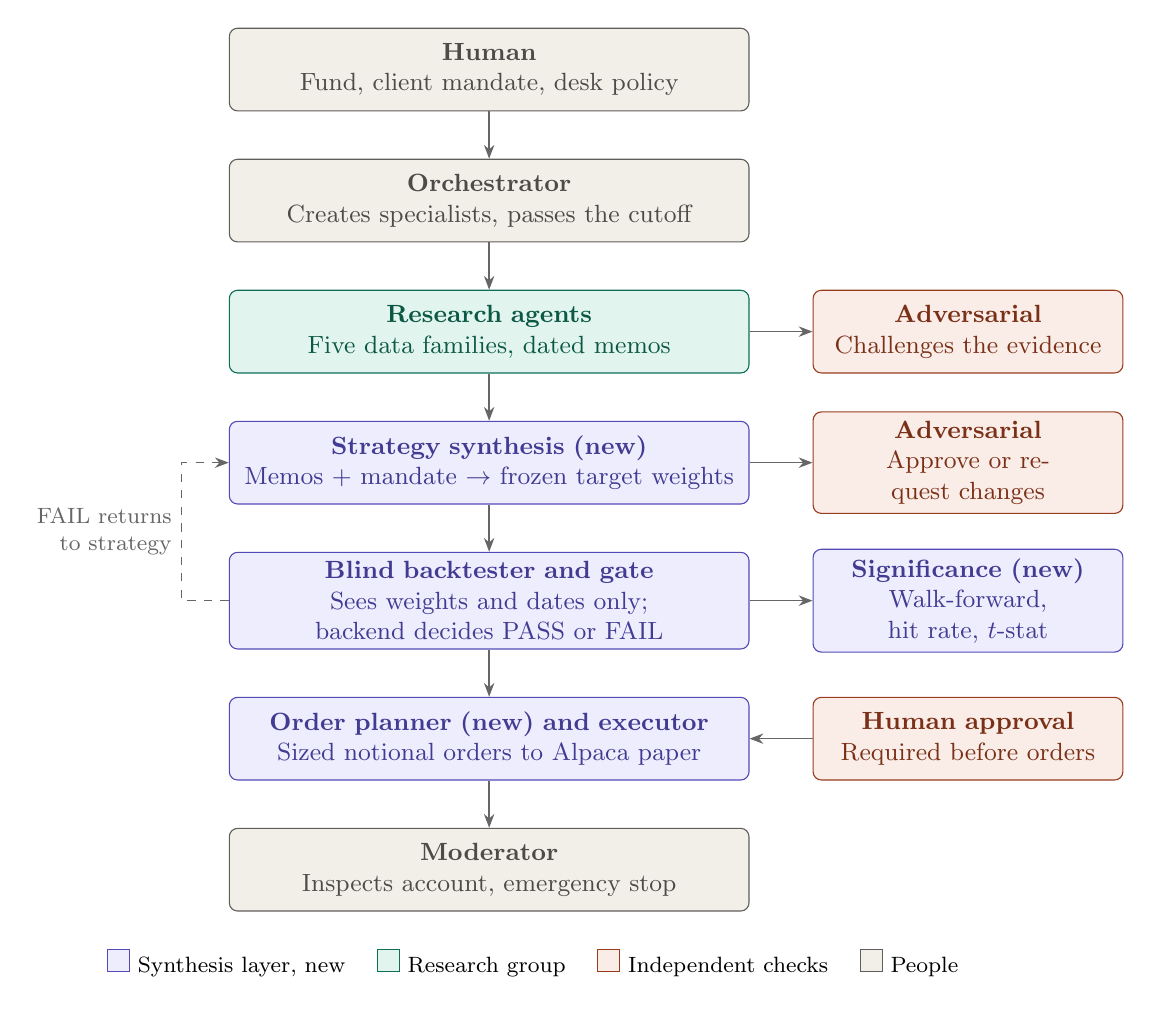
\begin{tikzpicture}[node distance=0.6cm and 0.8cm]
  \node[stage, hum] (human) {\textbf{Human}\\Fund, client mandate, desk policy};
  \node[stage, hum, below=of human] (orch) {\textbf{Orchestrator}\\Creates specialists, passes the cutoff};
  \node[stage, res, below=of orch] (research) {\textbf{Research agents}\\Five data families, dated memos};
  \node[stage, synth, below=of research] (strategy) {\textbf{Strategy synthesis (new)}\\Memos + mandate $\rightarrow$ frozen target weights};
  \node[stage, synth, below=of strategy] (gate) {\textbf{Blind backtester and gate}\\Sees weights and dates only; backend decides PASS or FAIL};
  \node[stage, synth, below=of gate] (exec) {\textbf{Order planner (new) and executor}\\Sized notional orders to Alpaca paper};
  \node[stage, hum, below=of exec] (mod) {\textbf{Moderator}\\Inspects account, emergency stop};

  \node[side, chk, right=of research] (adv1) {\textbf{Adversarial}\\Challenges the evidence};
  \node[side, chk, right=of strategy] (adv2) {\textbf{Adversarial}\\Approve or request changes};
  \node[side, synth, right=of gate] (sig) {\textbf{Significance (new)}\\Walk-forward, hit rate, $t$-stat};
  \node[side, chk, right=of exec] (appr) {\textbf{Human approval}\\Required before orders};

  \draw[flow] (human) -- (orch);
  \draw[flow] (orch) -- (research);
  \draw[flow] (research) -- (strategy);
  \draw[flow] (strategy) -- (gate);
  \draw[flow] (gate) -- (exec);
  \draw[flow] (exec) -- (mod);
  \draw[flow] (research) -- (adv1);
  \draw[flow] (strategy) -- (adv2);
  \draw[flow] (gate) -- (sig);
  \draw[flow] (appr) -- (exec);

  \draw[flow, dashed] (gate.west) -- ++(-0.6,0) |- node[pos=0.25, left, font=\footnotesize, align=right] {FAIL returns\\to strategy} (strategy.west);

  \node[below=0.35cm of mod, font=\footnotesize, align=left, xshift=0.6cm] (legend) {
    \tikz\node[draw=synth, fill=synthfill, minimum size=8pt, inner sep=0]{}; Synthesis layer, new \quad
    \tikz\node[draw=research, fill=researchfill, minimum size=8pt, inner sep=0]{}; Research group \quad
    \tikz\node[draw=check, fill=checkfill, minimum size=8pt, inner sep=0]{}; Independent checks \quad
    \tikz\node[draw=human, fill=humanfill, minimum size=8pt, inner sep=0]{}; People
  };
\end{tikzpicture}
\end{center}

\textbf{Gates the model cannot bypass.} A strategy must be registered (frozen) before review. The backtester is created only after an approving review and sees nothing but the weights and dates. The backend computes PASS or FAIL from human thresholds. Execution rechecks permission, PASS, review, approval, limits and the stop before every order. A submitted order is not a fill.

\newpage
\section*{2. Which variables each agent uses}

\small
\renewcommand{\arraystretch}{1.2}
\setlength{\LTleft}{0pt}\setlength{\LTright}{0pt}
\begin{longtable}{@{}R{2.2cm}R{4.4cm}R{4.4cm}R{4.2cm}@{}}
\toprule
\textbf{Agent} & \textbf{Reads} & \textbf{Produces} & \textbf{Bound by} \\
\midrule
\endfirsthead
\toprule
\textbf{Agent} & \textbf{Reads} & \textbf{Produces} & \textbf{Bound by} \\
\midrule
\endhead
\bottomrule
\endlastfoot
Research, live &
Financial Datasets statements, ratios, earnings, prices, filing sections, insider and institutional ownership, company news; Exa web search; X search; FRED series; Jev sentiment; Apify &
One memo per data family: ticker, stance (long, neutral, avoid), confidence 0 to 1, note, source ids with dates &
Live data never enters a historical decision \\
\addlinespace
Research, historical &
Cutoff-filtered snapshots: OHLCV closes; SEC revenue, net income, total debt keyed on filing date; FRED CPI, FEDFUNDS, DGS10, UNRATE keyed on release date; curated events and GDELT tone &
Same memo shape; every source dated on or before the cutoff &
\texttt{assert\_no\_lookahead} on every cited source \\
\addlinespace
\textbf{Strategy synthesis} (new) &
All memos; mandate universe, capital, risk band, max\_position, max\_drawdown; policy universe and max\_position &
Frozen strategy: name, weights summing to 1, cutoff, end, rationale, memo paths, changes\_my\_mind. Seed is 1 plus signed convictions; net-avoid names dropped; clamped to max\_position; optional single Bedrock refinement that is re-clamped in code &
\texttt{register\_strategy} rejects weights outside the universe or above max\_position; revisions get new ids \\
\addlinespace
Adversarial &
The research or the registered strategy, plus native evidence tools &
APPROVE or CHANGES\_REQUESTED with a critique &
Cannot review a strategy by its own author \\
\addlinespace
Backtester &
Only strategy id, weights, cutoff, end. The engine adds closes, SPY and the risk-free rate (FEDFUNDS at the cutoff) &
total\_return, cagr, max\_drawdown, sharpe for portfolio and SPY &
No file, web, research or delegation tools; bound to one strategy id \\
\addlinespace
Gate &
The metrics above; policy max\_drawdown, min\_sharpe, min\_excess\_return &
PASS or FAIL with per-check results and a policy hash &
Backend computes the verdict; a changed policy invalidates PASS \\
\addlinespace
\textbf{Significance} (new) &
Frozen weights; every monthly cutoff in range; fixed horizon &
Number of windows, hit rate vs SPY and equal weight, mean excess return, $t$-statistic, $p$-value, bootstrap 95\% interval &
Reported beside the gate, never replaces it; windows overlap, so the $t$-stat is optimistic \\
\addlinespace
\textbf{Order planner} (new) &
Weights; capital as the smaller of account equity and mandate capital; account cash, positions, open orders; max\_order\_notional, max\_daily\_orders &
Ordered list of buy and sell notional orders with stable client\_order\_ids, or blocked with a reason &
Sells before buys; nothing above cash, position cap or notional limit \\
\addlinespace
Executor &
The order plan; live web context only as a reason to defer &
Broker order id, status, filled\_qty, filled\_avg\_price &
Stop clear, trading\_allowed, current PASS, APPROVE, human approval and limits rechecked per order; an unknown result is never resubmitted \\
\addlinespace
Moderator &
Desk records, paper account, positions versus submitted orders &
\texttt{emergency\_stop} with a reason &
Can engage the stop; only a person clears it \\
\end{longtable}
\normalsize

\section*{3. How this maps onto the roles on \texttt{main}}

Kushagra's written role requirements take priority over the picture: the roster is flexible, one root can create more orchestrators and task-focused researchers, and the boxes above are context, not a fixed roster. The synthesis boxes are \textbf{tools on existing roles}, not new roles: \texttt{synthesize\_strategy} on the strategy role, \texttt{plan\_paper\_orders} and \texttt{execute\_order\_plan} on the executor role. The blind backtester implementation is Mayank's (lane 2b); synthesis hands it a frozen strategy record (weights, cutoff, end) by \texttt{strategy\_id} and consumes its PASS or FAIL. The significance report is an optional add-on and can be replaced by Mayank's walk-forward once it lands.

\section*{4. Limits to state in the demo}
\begin{itemize}[leftmargin=1.2em, itemsep=2pt]
  \item Historical evaluation is the recorded monthly target-weight engine on cached closes: no dividends, no costs, fully invested. Significance is a walk-forward over cutoffs with the same frozen weights, which measures robustness of the allocation, not of a live rebalancing process.
  \item Live provider data is not point-in-time safe and never feeds a historical decision.
  \item Hiding research from the evaluator does not remove model-memory leakage; see Mayank's \path{docs/track3-plan.md} for the masked-ticker audit.
  \item Alpaca paper is a shared account; a submitted order is not a fill.
\end{itemize}
\end{document}
